El desarrollo de la aplicación web ``LogArt: Galería de Recuerdos'' se ha fundamentado en un conjunto cuidadosamente seleccionado de tecnologías modernas, herramientas de desarrollo eficientes y una metodología de trabajo estructurada. 

Este capítulo tiene como objetivo describir en detalle cada uno de estos componentes, justificando las elecciones realizadas y explicando su papel en la consecución de los objetivos del proyecto.

La naturaleza de LogArt, una aplicación web interactiva y centrada en el usuario, demandaba un stack tecnológico que ofreciera flexibilidad, un alto rendimiento y una experiencia de desarrollo productiva. Por este motivo, se optó por el stack \textbf{MERN (MongoDB, Express.js, React, Node.js)}. 

Aunque en entornos corporativos de gran escala son frecuentes las arquitecturas basadas en lenguajes de tipado estricto como Java con Spring Boot y frameworks como Angular, la adopción del ecosistema MERN responde a estándares de la industria ampliamente consolidados en el desarrollo de aplicaciones modernas y ágiles. Esta elección se considera especialmente idónea para LogArt debido a varios factores estratégicos: la agilidad que proporciona el uso de JavaScript de forma isomórfica en todo el stack (Fullstack JavaScript), la flexibilidad del esquema de MongoDB para la gestión de datos heterogéneos, y el robusto ecosistema de React para la creación de interfaces de usuario altamente dinámicas. De este modo, la arquitectura propuesta no solo cumple con los requisitos técnicos del proyecto, sino que se alinea con las tendencias tecnológicas actuales de alto rendimiento. Esta decisión se detalla con mayor profundidad en la Sección~\ref{sec:stackMERN}.

Complementando el stack principal, se han integrado herramientas de \textit{DevOps} cruciales como \textbf{Docker} y \textbf{Docker Compose} para la contenedorización de la aplicación, garantizando entornos de desarrollo y despliegue consistentes y portables (ver Sección \ref{sec:contenedores}).


Asimismo, se ha implementado un flujo de \textbf{Integración Continua y Entrega Continua (CI/CD)} utilizando \textbf{GitHub Actions}. Este sistema automatiza la ejecución de las pruebas y la publicación de nuevas versiones mediante imágenes de Docker, lo que garantiza que el software esté siempre en un estado reproducible y listo para su distribución. Este enfoque ha contribuido significativamente a la calidad y eficiencia del ciclo de desarrollo (detallado en la Sección~\ref{sec:cicd}).

Desde el punto de vista metodológico, el proyecto ha seguido un enfoque \textbf{iterativo e incremental}, fundamentado en las buenas prácticas de la ingeniería del software y los marcos de trabajo ágiles ampliamente aceptados en la industria tecnológica actual. Este enfoque ha permitido construir la aplicación de forma progresiva, mediante ciclos de desarrollo que culminan en entregas funcionales parciales. Esta estrategia ha facilitado la validación continua de los hitos alcanzados, permitiendo una adaptación ágil ante requisitos emergentes o ajustes técnicos necesarios durante el proceso. La gestión del proyecto se ha apoyado en herramientas de planificación profesional como \textbf{GitHub Projects} y una comunicación constante con el tutor, elementos clave para asegurar un seguimiento riguroso del trabajo y el cumplimiento de los estándares de calidad exigidos, tal como se describe en la Sección~\ref{sec:metodologiaDesarrollo}.

El conjunto de estas decisiones metodológicas ha conformado un marco de trabajo robusto sobre el que se ha edificado LogArt, buscando un equilibrio entre la innovación tecnológica, la mantenibilidad del software y los principios fundamentales del desarrollo profesional de aplicaciones web.

A modo de resumen visual a alto nivel, la Figura~\ref{fig:stack_tecnologico} ilustra la arquitectura tecnológica del proyecto clasificada por capas, mientras que la Tabla~\ref{tab:resumen_tecnologias} proporciona una descripción concisa de cada una de las herramientas adoptadas.

\begin{figure}[hbt!]
    \centering
    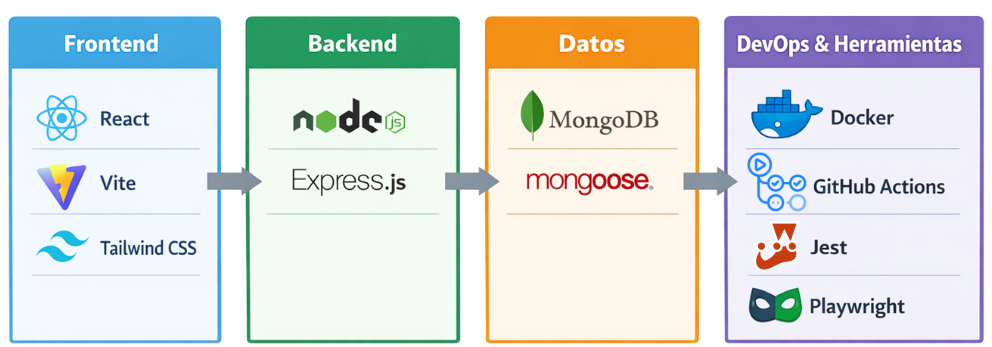
\includegraphics[width=0.9\textwidth]{img/stack_tecnologico.png}
    \caption{Visión de alto nivel del stack tecnológico y herramientas del proyecto.}
    \label{fig:stack_tecnologico}
\end{figure}

\begin{table}[hbt!]
\centering
\renewcommand{\arraystretch}{1.3}
\begin{tabular}{|l|l|p{9cm}|}
\hline
\textbf{Categoría} & \textbf{Tecnología} & \textbf{Descripción Principal} \\ \hline
\multirow{3}{*}{\textbf{Frontend}} & React & Librería para la construcción de la interfaz de usuario (SPA). \\ \cline{2-3} 
 & Vite & Herramienta de construcción y servidor de desarrollo ultrarrápido. \\ \cline{2-3} 
 & Tailwind CSS & Framework CSS de utilidades para el diseño visual. \\ \hline
\multirow{2}{*}{\textbf{Backend}} & Node.js & Entorno de ejecución de JavaScript del lado del servidor. \\ \cline{2-3} 
 & Express.js & Framework minimalista para la creación de la API RESTful. \\ \hline
\multirow{2}{*}{\textbf{Base de Datos}} & MongoDB & Sistema de gestión de bases de datos NoSQL orientado a documentos. \\ \cline{2-3} 
 & Mongoose & Librería ODM para el modelado y validación de datos en MongoDB. \\ \hline
\multirow{3}{*}{\textbf{DevOps \& Infra.}} & Docker & Plataforma para la contenedorización de la aplicación. \\ \cline{2-3} 
 & GitHub Actions & Servicio para la automatización de pipelines de CI/CD. \\ \cline{2-3} 
 & Git / GitHub & Sistema de control de versiones y plataforma de alojamiento. \\ \hline
\multirow{3}{*}{\textbf{Pruebas}} & Jest & Framework de pruebas para tests unitarios y de integración. \\ \cline{2-3} 
 & Supertest & Librería para la simulación y prueba de peticiones HTTP a la API. \\ \cline{2-3} 
 & Playwright & Framework para la automatización de pruebas End-To-End (E2E). \\ \hline
\end{tabular}
\caption{Resumen descriptivo de las tecnologías y herramientas utilizadas.}
\label{tab:resumen_tecnologias}
\end{table}

\section{Stack Tecnológico: MERN}
\label{sec:stackMERN}

La elección del stack tecnológico es una decisión crucial en cualquier proyecto de desarrollo de software, ya que impacta directamente en la productividad, el rendimiento, la escalabilidad y el mantenimiento de la aplicación. Para LogArt, se optó por el stack MERN, un acrónimo que representa cuatro tecnologías clave (y de código abierto) basadas en JavaScript: \textbf{M}ongoDB, \textbf{E}xpress.js, \textbf{R}eact y \textbf{N}ode.js. Esta combinación permite el desarrollo de aplicaciones FullStack utilizando JavaScript tanto en el lado del cliente como en el del servidor, lo que ofrece multitud de ventajas\cite{adityabhuyanMERNAdvantages}, siendo la reutilización de conocimientos la principal ventaja en un TFG como este, donde una sola persona desarrolla una aplicación entera de principio a fin.

La adopción del stack MERN para LogArt se justifica por su popularidad en la industria para la creación de aplicaciones web modernas, su gran comunidad de desarrolladores, la abundancia de recursos y librerías disponibles, y su idoneidad para proyectos que requieren agilidad y un desarrollo rápido de prototipos funcionales. A continuación, se describen los componentes de este stack y otras tecnologías fundamentales empleadas en el \textit{backend} y \textit{frontend} de LogArt.

\subsection{Backend}
\label{sec:backendTech}

El \textit{backend} de LogArt es el responsable de la lógica de negocio, la gestión de datos, la autenticación de usuarios y la exposición de una API RESTful para la comunicación con el \textit{frontend}. Las tecnologías principales utilizadas se detallan a continuación:

\subsubsection{Node.js}
\label{sec:nodejs}

\begin{itemize}
    \item \textbf{¿Qué es?:} Node.js\footnote{\url{https://nodejs.org/}} es un entorno de ejecución de JavaScript del lado del servidor, asíncrono y orientado a eventos, construido sobre el motor V8 de JavaScript de Google Chrome. Permite a los desarrolladores construir aplicaciones de red escalables y de alto rendimiento \cite{kinstaQueEsNodeJS}.

    \item \textbf{¿Por qué se eligió para LogArt?:}
        \begin{itemize}
            \item \textit{Fullstack JavaScript:} La principal ventaja fue la posibilidad de utilizar JavaScript tanto en el \textit{backend} como en el \textit{frontend} (con React), lo que simplifica el contexto de desarrollo y permite una mayor sinergia.
            \item \textit{Rendimiento para I/O:} Su modelo de I/0 (Entrada/Salida) no bloqueante lo hace eficiente para aplicaciones que manejan múltiples conexiones concurrentes y operaciones intensivas de I/O, como es el caso de una aplicación web que interactúa constantemente con una base de datos.
            \item \textit{Ecosistema NPM:} Node Package Manager (NPM) proporciona acceso a un vasto repositorio de módulos y librerías de código abierto que aceleran el desarrollo, como Express.js para el framework web o Mongoose para la interacción con MongoDB.
            \item \textit{Comunidad y Curva de Aprendizaje:} Al ser una tecnología ampliamente adoptada, existe una gran cantidad de documentación, tutoriales y soporte comunitario. Para un proyecto de TFG, donde el tiempo es un factor, una curva de aprendizaje manejable es muy beneficiosa.
        \end{itemize}
    \item \textbf{¿Cómo se usó específicamente en LogArt?:}
    En LogArt, Node.js constituye la base sobre la cual se ejecuta todo el servidor de la aplicación. Se utiliza para:
        \begin{itemize}
            \item Ejecutar el framework Express.js para definir y gestionar las rutas de la API.
            \item Conectar con la base de datos MongoDB a través de la librería Mongoose.
            \item Implementar la lógica de negocio para las operaciones CRUD (Crear, Leer, Actualizar, Eliminar) sobre las entidades de la aplicación (usuarios, objetos, comentarios, etc.).
            \item Gestionar la autenticación de usuarios mediante tokens JWT.
            \item Servir como plataforma para ejecutar las pruebas automatizadas del \textit{backend} con Jest y Supertest.
        \end{itemize}
    \item \textbf{Versión:} Se utilizó la versión LTS (Long Term Support) \textbf{v20.18.0} de Node.js.
\end{itemize}

\subsubsection{Express.js}
\label{sec:expressjs}

\begin{itemize}
    \item \textbf{¿Qué es?:} Express.js\footnote{\url{https://expressjs.com/}} es un framework de aplicaciones web para Node.js, minimalista, bastante flexible y de código abierto también. Proporciona un conjunto robusto de características para desarrollar aplicaciones web y APIs, sin imponer una estructura ``rígida'', lo que permite a los desarrolladores una gran libertad en la organización del proyecto \cite{kinstaQueEsExpress}.
    \item \textbf{¿Por qué se eligió para LogArt?:}
        \begin{itemize}
            \item \textit{Entandar de facto para Node.js} Es el framework más popular y ampliamente utilizado en el ecosistema Node.js para la construcción de \textit{backends} y APIs, lo que se traduce en una vasta cantidad de documentación, tutoriales y soluciones a problemas comunes.
            \item \textit{Minimalismo y Flexibilidad:} Su naturaleza ``unopinionated'' permite construir la aplicación añadiendo solo las funcionalidades necesarias a través de \textit{middleware}, lo que resulta en una aplicación mucho más ligera y adaptada a los requisitos específicos de LogArt.
            \item \textit{Gestión de Rutas y Peticiones HTTP:} Simplifica la definición de rutas para la API, el manejo de diferentes métodos HTTP (GET, POST, PUT, DELETE, etc) y el procesamiento de los datos de las peticiones.
            \item \textit{Integración con Middleware:} Facilita la incorporación de \textit{middleware} para tareas comunes como el parseo del cuerpo de las peticiones (ej. \texttt{express.json()}, la gestión de errores, la seguridad (ej. \texttt{cors}), o la autenticación con JWT.
        \end{itemize}
    \item \textbf{¿Cómo se usó específicamente en LogArt?:}
    En el \textit{backend} de LogArt, Express.js es el pilar fundamental sobre el que se construye la API RESTful. Sus usos principales son:
        \begin{itemize}
            \item \textbf{Definición de Rutas (Routing):} Se utiliza el sistema de enrutamiento de Express para mapear las URLs de la API (endpoints) a los controladores específicos que manejan la lógica para cada recurso (ej. \texttt{api/v1/users}, \texttt{api/v1/objects}, \texttt{api/v1/auth}...).
            \item \textbf{Manejo de Peticiones y Respuestas:} Procesa las peticiones HTTP entrantes, extrae parámetros, datos del cuerpo (body) y cabeceras (headers), y construye las respuestas HTTP correspondientes, incluyendo códigos de estado y cuerpos de respuesta en formato JSON.
            \item \textbf{Integración de Middleware:}
                \begin{itemize}
                    \item \texttt{cors}: Para habilitar el Intercambio de Recursos de Origen Cruzado (CORS), permitiendo que el \textit{frontend} (servido desde un origen diferente en desarrollo) pueda realizar peticiones al \textit{backend}.
                    \item \texttt{express.json()}: Para parsear el cuerpo de las peticiones en formato JSON.
                    \item Middleware personalizado para la autenticación con JWT, verificando los tokens en las cabeceras de las peticiones para proteger rutas.
                \end{itemize}
            \item \textbf{Organización de la API:} Aunque Express es minimalista, como se ha comentado antes, ha permitido sin embargo estructurar la API de LogArt de forma modular, separando las rutas y controladores por entidad/funcionalidad.
        \end{itemize}
    \item \textbf{Versión:} Se utilizó la versión \textbf{v4.21.1} de Express.js.
\end{itemize}

\subsubsection{MongoDB}
\label{sec:mongodb}

\begin{itemize}
    \item \textbf{¿Qué es?:} MongoDB\footnote{\url{https://www.mongodb.com/}} es un sistema de gestión de bases de datos NoSQL de código abierto, orientado a documentos. En lugar de almacenar datos en tablas con filas y columnas como las bases de datos relacionales tradicionales, MongoDB almacena datos en colecciones de documentos flexibles en formato BSON (Binary JSON), que es una representación binaria de JSON \cite{aprenderbigdataMongoDB}.
    \item \textbf{¿Por qué se eligió para LogArt?:}
        \begin{itemize}
            \item \textit{Flexibilidad de Esquema (Schema-less):} Una de las principales razones para elegir MongoDB fue su flexibilidad. Al ser LogArt una aplicación que maneja diversos tipos de ``recuerdos'' y obras (libros, videojuegos, canciones), cada uno con atributos potencialmente diferentes o que podrían evolucionar (como acabó pasando), un esquema flexible es muy ventajoso. Permite añadir nuevos campos o modificar la estructura de los datos sin necesidad de migraciones de esquema complejas como en las bases de datos SQL.
            \item \textit{Herramientas Complementarias para el Desarrollo y Despliegue:} Durante el desarrollo, se utilizó MongoDB Compass como interfaz gráfica para explorar y depurar los datos de forma visual, lo cual agilizó mucho las tareas de prueba y validación de los datos que se iban añadiendo/eliminando/modificando. Además, se usó también al comienzo una instancia de MongoDB Atlas, como servicio de base de datos en la nube, alojando la base de datos en un cluster accesible desde la web, lo que permitió pruebas remotas, sin ningún tipo de instalación.
            \item \textit{Escalabilidad Horizontal:} MongoDB está diseñado para escalar horizontalmente (``scale-out'') mediante técnicas como el \textit{sharding}, lo que sirve para distribuir los datos a través de múltiples servidores. Aunque para la escala de la aplicación del TFG esto no es un requisito inmediato, es una característica importante para el crecimiento a futuro de cualquier aplicación.
            \item \textit{Buen Rendimiento para Cargas de Trabajo Específicas:} Para muchas operaciones comunes en aplicaciones web, como consultas por múltiples criterios, o el manejo de datos semi-estructurados, MongoDB ofrece un buen rendimiento.
            \item \textit{Integración Nativa con JavaScript/Node.js:} Almacenar datos en un formato similar a JSON (BSON) facilita la interacción desde las propias aplicaciones JavaScript/Node.js, ya que los datos pueden mapearse de forma natural a objetos JavaScript sin necesidad de transformaciones ORM (Object-Relational Mapping). Sin embargo, para añadir estructura, validación y una capa más de modelado más robusta, se utilizó Mongoose, una librería ODM (Object Data Modeling) que permite definir esquemas y modelos en Node.js sobre MongoDB.
            \item \textit{Comunidad y Ecosistema:} MongoDB cuenta con una amplia comunidad, extensiva documentación y herramientas de desarrollo como las ya mencionadas anteriormente (MongoDB Compass y Atlas) que facilitan su uso.
        \end{itemize}
    \item \textbf{¿Cómo se usó específicamente en LogArt?:}
    En LogArt, MongoDB actúa como el sistema de persistencia principal. Se encarga de almacenar toda la información vital del sistema, estructurada en colecciones para usuarios, objetos, comentarios, disciplinas y control de seguridad (tokens invalidados). El diseño específico de estas colecciones y el modelo de datos subyacente se detallan en el Capítulo~\ref{chap:descripcionInformatica}. Se interactúa con la base de datos desde el \textit{backend} a través de la librería Mongoose.
    \item \textbf{Versión:} Se utilizó la versión \textbf{v7+} de MongoDB.
\end{itemize}

\subsubsection{Mongoose}
\label{sec:mongoose}

\begin{itemize}
    \item \textbf{¿Qué es?:} Mongoose\footnote{\url{https://mongoosejs.com/}} es una librería ODM (Object Data Modeling) para MongoDB y Node.js. Proporciona una solución elegante y basada en esquemas para modelar los datos de la aplicación, ofreciendo una capa de abstracción sobre las interacciones directas con la base de datos MongoDB \cite{freecodecampMongooseIntro}.

    \item \textbf{¿Por qué se eligió para LogArt?:}
        \begin{itemize}
            \item \textit{Modelado de Datos Estructurados:} Aunque MongoDB es flexible en su esquema, Mongoose permite definir esquemas a nivel de aplicación. Esto es crucial para LogArt para asegurar la consistencia de los datos, definir tipos de datos para cada campo, establecer valores por defecto y crear validaciones.
            \item \textit{Validación de Datos:} Incorpora un sistema de validación robusto que permite definir reglas para los datos antes de que se guarden en la base de datos (ej. campos requeridos, tipos de datos, expresiones regulares, etc), ayudando a mantener la integridad de la información.
            \item \textit{Funcionalidades de Middleware y Hooks:} Permite definir funciones que se ejecutan antes o después de ciertas operaciones (ej. antes de guardar un documento - \texttt{pre-('save')} - para hashear una contraseña, o después de encontrar un documento).
            \item \textit{Población de Referencias (\texttt{populate}):} Simplifica la tarea de traer datos de colecciones relacionadas. Por ejemplo, al obtener un ``objeto'' de LogArt, Mongoose puede ``poblar'' automáticamente la información del usuario propietario o los comentarios asociados a ese objeto, que residen en colecciones separadas.
            \item \textit{Sintaxis Intuitiva para Consultas:} Ofrece una API fluida y encadenable para construir consultas completas a MongoDB, haciendo el código más legible y mantenible.
            \item \textit{Simplificación de la Interacción con MongoDB:} Abstrae muchas de las complejidades de la API nativa de MongoDB, facilitando la conexión a la base de datos, la gestión de modelos y la ejecución de las operaciones CRUD
        \end{itemize}
        
    \item \textbf{¿Cómo se usó específicamente en LogArt?:} Mongoose es una pieza central en la capa de acceso a datos del \textit{backend} de LogArt:
        \begin{itemize}
            \item \textbf{Definición de Esquemas y Modelos:} Se crearon esquemas Moongose para cada una de las entidades principales de la aplicación: \texttt{User}, \texttt{Object}, \texttt{Comment}, \texttt{Discipline}, \texttt{BlacklistedToken}. Estos esquemas definen la estructura, los tipos de datos (String, Number, Date, ObjectId, etc), los campos requeridos y las validaciones para cada entidad. A partir de estos esquemas, se crearon modelos Mongoose que representan las colecciones en MongoDB y proporcionan la interfaz para interactuar con ellas.
            \item \textbf{Operaciones CRUD:} Todas las operaciones de creación, lectura, actualización y eliminación de datos en MongoDB se realizan a través de los modelos Mongoose (ej. \texttt{User.create()}, \texttt{Object.findById()}, \texttt{Comment.updateOne()}, \texttt{Object.deleteOne()}).
            \item \textbf{Validaciones:} Se utilizaron las capacidades de validación de Mongoose para asegurar, por ejemplo que el email de un usuario se guarde en minúsculas, que ciertos campos sean obligatorios al crear un objeto, o que la biografía tenga un límite de caracteres.
            \item \textbf{Población de Datos Relacionados:} Se utilizó la función \texttt{populate()} para cargar eficientemente datos referenciados. Por ejemplo, al mostrar los detalles de un \texttt{Object}, se poblaron los datos del \texttt{User} que lo creó.
        \end{itemize}
    \item \textbf{Versión:} Se utilizó la versión \textbf{v8.8.3} de Mongoose.
\end{itemize}

\subsubsection{Autenticación y Seguridad}
\label{sec:authSeguridadBackend}

Garantizar la seguridad de los datos de los usuarios y proteger el acceso a la aplicación son aspectos fundamentales en el desarrollo de LogArt. Para ello, se implementaron mecanismos de autenticación y gestión segura de credenciales usando las siguientes tecnologías:

\begin{itemize}
    \item \textbf{JSON Web Tokens (JWT}
        \begin{itemize}
            \item \textbf{¿Qué es?:} JSON Web Token (JWT)\footnote{\url{https://datatracker.ietf.org/doc/html/rfc7519}} es un estándar abierto (RFC 7519)\cite{rfc7519} que define una forma compacta y autocontenida para transmitir información de forma segura entre partes como un objeto JSON. Esta información puede ser verificada y confiable porque está firmada digitalmente. Los JWTs se pueden firmar usando un secreto (con el algoritmo HMAC) o un par de claves pública/privada (usando RSA o ECDSA) \cite{caronteJWT}.
            \item \textbf{¿Por qué se eligió para LogArt?:}
                \begin{itemize}
                    \item \textit{Autenticación Stateless (con matices):} Los JWTs permiten, en teoría, implementar un sistema de autenticación sin estado (stateless) en el servidor, ya que el token contiene de forma autocontenida la información del usuario. Sin embargo, cabe señalar que para mejorar la seguridad en LogArt y permitir el cierre de sesión, se ha implementado una lista negra (\textit{blacklist}) de tokens invalidados en la base de datos. Esto introduce un componente de estado en el proceso de verificación, pues el servidor debe consultar dicha lista para asegurar que el token no ha sido revocado antes de su expiración, equilibrando así la escalabilidad de los JWT con un control de acceso más riguroso.
                    \item \textit{Ampliamente Adoptado y Estándar:} Es un estándar muy utilizado en la industria para la autenticación en APIs RESTful y aplicaciones web modernas.
                    \item \textit{Seguridad} Cuando se firman con un secreto robusto y se transmiten sobre HTTPS, los JWTs son una forma segura de manejar la autenticación. Pueden contener además \textit{claims} (información) sobre el usuario, como su ID o rol, lo que facilita la autorización.
                    \item \textit{Compatibilidad:} Son fáciles de usar en diferentes plataformas y lenguajes, siendo ideales para la comunicación entre el \textit{frontend} React y el \textit{backend} Node.js de LogArt.
                \end{itemize}
            \item \textbf{¿Cómo se usó específicamente en LogArt?:} El flujo de autenticación es el siguiente:
            \begin{itemize}
                \item \textbf{Inicio de Sesión:} Cuando un usuario inicia sesión con sus credenciales (email y contraseña), el \textit{backend} verifica estas credenciales contra la base de datos.
                \item \textbf{Generación del Token:} Si las credenciales son válidas, el servidor genera un JWT que contiene un \textit{payload} con información del usuario (ej. \texttt{userId}). Este token se firma utilizando un secreto almacenado de forma segura en las variables de entorno del servidor.
                \item \textbf{Envío al Cliente:} El JWT generado se envía al cliente (\textit{frontend} React) en la respuesta del inicio de sesión.
                \item \textbf{Almacenamiento en el Cliente:} El \textit{frontend} almacena el JWT (en \texttt{storageState}).
                \item \textbf{Autorización de Peticiones:} para las rutas protegidas de la API, el \textit{frontend} incluye el JWT en la cabecera \texttt{Authorization} de cada petición (con el prefijo \texttt{Bearer}.
                \item \textbf{Verificación en el Servidor:} Un middleware en el \textit{backend} intercepta estas peticiones, extrae el JWT de la cabecera y verifica su firma utilizando el mismo secreto. Si el token es válido y no ha expirado, se permite el acceso al recurso solicitado; de lo contrario, se devuelve un error de no autorizado.
            \end{itemize}
        Se utilizó la librería \texttt{jsonwebtoken} para la generación y verificación de los tokens.
        \item \textbf{Versión (jsonwebtoken):} Se utilizó la versión \textbf{v9.0.2}
        \end{itemize}
        \vspace{0.5cm}

        \item  \textbf{Bcrypt}
            \begin{itemize}
                \item \textbf{¿Qué es?:} Bcrypt\footnote{\url{https://www.npmjs.com/package/bcrypt}} es una función de derivación de claves basada en el cifrado Blowfish, diseñada para el hashing de contraseñas \cite{webempresaBcrypt}.
                \item \textbf{¿Por qué se eligió para LogArt?:}
                    \begin{itemize}
                        \item \textit{Seguridad en el Almacenamiento de Contraseñas:} Es fundamental no almacenar contraseñas en texto plano, y Bcrypt es uno de los algoritmos de hashing más recomendados y seguros para contraseñas porque es lento por diseño (dificultando ataques de fuerza bruta) e incluye un \textit{salt} (una cadena aleatoria) para cada contraseña antes de hashearla, lo que protege contra ataques de varios tipos.
                        \item \textit{Estándar de la Industria:} Es una práctica estándar y recomendada en la industria para la protección de contraseñas.
                    \end{itemize}
            \item \textbf{¿Cómo se usó específicamente en LogArt?:}
                \begin{itemize}
                    \item \textbf{Hashing de Contraseñas en el Registro:} Cuando un nuevo usuario se registra en LogArt, su contraseña no se guarda directamente. En su lugar, se utiliza Bcrypt para generar un \texttt{salt} aleatorio y luego se hashea la contraseña junto con este \texttt{salt}. El hash resultante es lo que se almacena en el campo contraseña del documento del usuario en MongoDB.
                    \item \textbf{Verificación de Contraseñas en el Inicio de Sesión:} Cuando un usuario intenta iniciar sesión, proporciona su contraseña en texto plano. El \textit{backend} recupera el hash almacenado para ese usuario de la base de datos. Luego Bcrypt se utiliza para comparar la contraseña proporcionada con el hash almacenado. La función de comparación de Bcrypt internamente extrae el \texttt{salt} del hash y vuelve a hashear la contraseña proporcionada para ver si coincide, sin necesidad de almacenar el \texttt{salt} por separado.
                \end{itemize}
            Se utilizó la librería \texttt{bcrypt}
            \item \textbf{Versión (\texttt{bcrypt}):} Se utilizó la versión \textbf{v5.1.1}
            \end{itemize}
\end{itemize}

\subsection{Frontend}
\label{sec:frontendTech}

El \textit{frontend} de LogArt es la interfaz con la que el usuario interactúa directamente. Se ha desarrollado como una \textit{Single Page Application} (SPA) para ofrecer una experiencia de usuario fluida, atractiva y dinámica. Las tecnologías clave son:

\subsubsection{React}
\label{sec:react}

    \begin{itemize}
        \item \textbf{¿Qué es?:} React\footnote{\url{https://react.dev/}} es una biblioteca de JavaScript de código abierto, desarrollada por Facebook, para construir interfaces de usuario interactivas y re-utilizables basadas en componentes \cite{kinstaQueEsReactJS}.

        \item \textbf{¿Por qué se eligió para LogArt?:}
        \begin{itemize}
            \item \textit{Desarrollo Basado en Componentes:} Permite dividir la UI en componentes independientes y re utilizables, facilitando la gestión y escalabilidad de la interfaz de LogArt.
            \item \textit{Virtual DOM:} Optimiza las actualizaciones del DOM real, mejorando el rendimiento y la fluidez de la aplicación, especialmente con listas dinámicas de objetos y comentarios.
            \item \textit{Ecosistema y Comunidad:} Amplia disponibilidad de librerías complementarias (para enrutamiento, gestión de estado, etc.) y un fuerte soporte comunitario.
            \item \textit{Declaratividad:} Facilita la creación de UIs complejas al describir cómo deberían lucir en diferentes estados, encargándose React de las actualizaciones.
        \end{itemize}
    \item \textbf{¿Cómo se usó específicamente en LogArt?:} React es la base de toda la interfaz de usuario en LogArt. Se ha utilizado para:
        \begin{itemize}
            \item \textbf{Construir todos los componentes visuales:} Desde elementos básicos como botones y campos de entrada, hasta vistas complejas como la galería de objetos, los formularios de creación/edición, y el perfil de usuario.
            \item \textbf{Gestionar el Estado:} Gestionar el estado local de los componentes (ej. datos de formularios, visibilidad de modales, etc).
            \item \textbf{Eventos de usuario:} Manejar eventos de usuario (clics, entradas de texto) para interactuar con la lógica de la aplicación
            \item \textbf{API:} Consumir la API RESTful del \textit{backend} mediante Axios para obtener y enviar datos.
            \item \textbf{Navegación:} Implementar la navegación entre las diferentes secciones de la aplicación utilizando React Router DOM.
        \end{itemize}
    Se hizo un uso extensivo uso de los \textit{hooks} de React (ej. \texttt{useState}, \texttt{useEffect}, \texttt{useContext} para la gestión del estado y el ciclo de vida de los componentes.
    \item \textbf{Versión:} Se utilizó la versión \textbf{v18.3.1} de React.
\end{itemize}

\subsubsection{Vite}
\label{sec:vite}

    \begin{itemize}
        \item \textbf{¿Qué es?:} Vite\footnote{\url{https://vitejs.dev}} es una herramienta de construcción de \textit{frontend} moderna y muy rápida. Proporciona un servidor de desarrollo con un arranque casi instantáneo y Hot Module Replacement (HMR) muy eficiente, además de optimizar los builds para producción \cite{viteWhy}.
        \item \textbf{¿Por qué se eligió para LogArt?:}
            \begin{itemize}
                \item \textit{Velocidad de Desarrollo:} Su principal atractivo es la mejora significativa en la velocidad del servidor de desarrollo y las actualizaciones HMR en comparación con herramientas más antiguas como Webpack (usado por Create React App). Esto agiliza notablemente el ciclo de desarrollo.
                \item \textit{Configuración Sencilla:} Ofrece una configuración por defecto muy completa para proyectos React, reduciendo la necesidad de configuraciones complejas.
                \item \textit{Builds Optimizados:} Para producción, Vite utiliza Rollup bajo el capó, generando bundles optimizados y eficientes.
            \end{itemize}
        \item \textbf{¿Cómo se usó específicamente en LogArt?:} Vite se utilizó como la herramienta de construcción y servidor de desarrollo para el \textit{frontend} de LogArt:
            \begin{itemize}
                \item \textbf{Servidor de Desarrollo:} Proporcionó el entorno de desarrollo local donde se construyó y probó la interfaz de React, beneficiándose de su rápido HMR para ver los cambios reflejados instantáneamente en el navegador.
                \item \textbf{Proceso de Build:} Se utilizó el comando \texttt{vite build} para generar los archivos estáticos optimizados del \textit{frontend} (HTML, CSS, JavaScript) que luego son servidos por el \textit{backend}.
                \item \textbf{Gestión de Módulos ES Nativos:} Aprovecha los módulos nativos del navegador durante el desarrollo, lo que contribuye a su velocidad.
            \end{itemize}
        \item \textbf{Versión:} Se utilizó la versión \textbf{v6.0.1} de Vite.
    \end{itemize}

\subsubsection{Gestión de Rutas y Peticiones HTTP}
\label{sec:rutasPeticionesFrontend}

Para la navegación dentro de la \textit{Single Page Application} (SPA) y la comunicación con el \textit{backend}, se emplearon las siguientes librerías:

\begin{itemize}
    \item \textbf{React Routes DOM}
        \begin{itemize}
            \item \textbf{¿Qué es?:} React Routes DOM\footnote{\url{https://reactrouter.com}} es la librería estándar para el enrutamiento en aplicaciones React. Permite definir rutas navegables, gestionar el historial del navegador y renderizar componentes específicos según la URL actual \cite{urianvieraReactRouterDomGuia}.
            \item \textbf{Uso en LogArt:} Se utilizó para definir las diferentes ``páginas'' o vistas de la aplicación (ej. \texttt{/}, \texttt{/login}, \texttt{/register}, \texttt{/profile}, etc), permitiendo a los usuarios navegar entre ellas sin recargar la página completa. Se emplearon componentes como \texttt{<Routes>}, \texttt{<Route>} y hooks como \texttt{useNavigate()} y \texttt{useParams()}.
            \item \textbf{Versión:} Se utilizó la versión \textbf{v6.26.1}.
        \end{itemize}
    \vspace{0.3cm}
    \item \textbf{Axios}
        \begin{itemize}
            \item \textbf{¿Qué es?:} Axios\footnote{\url{https://axios-http.com/}} es un cliente HTTP basado en promesas, muy popular para realizar peticiones AJAX desde el negador o desde Node.js. Simplifica la comunicación con APIs RESTful \cite{desarrollowebAxios}.
            \item \textbf{Uso en LogArt:} Se utilizó para todas las interacciones del \textit{frontend} con la API REST del \textit{backend} de LogArt, incluyendo autenticación de usuarios, la obtención de datos de objetos y comentarios, y el envío de nueva información o actualizaciones. Permitió manejar fácilmente las respuestas y errores de las peticiones de forma asíncrona. Se configuró una instancia de Axios para incluir automáticamente el token JWT en las cabeceras de las peticiones a rutas protegidas.
            \item \textbf{Versión:} Se utilizó la versión \textbf{v1.7.8}.
        \end{itemize}
\end{itemize}

\subsubsection{Estilos e Interfaz de Usuario (UI)}
\label{sec:estilosUiFrontend}

Para la apariencia visual, la experiencia de usuario y la interactividad de la interfaz de LogArt, se utilizaron las siguientes herramientas y librerías:

    \begin{itemize}
        \item \textbf{Tailwind CSS}
            \begin{itemize}
                \item \textbf{¿Qué es?:} Tailwind\footnote{\url{https://tailwindcss.com/}} es un framework CSS ``utility-first'' que proporciona clases de bajo nivel altamente componibles para construir diseños personalizados directamente en el marcado HTML (JSX en este caso), sin necesidad de escribir CSS convencional \cite{vabadusTailwindIntro}.
                \item \textbf{Uso en LogArt:} Se empleó extensivamente para estilizar todos los componentes de React, permitiendo un desarrollo ágil de la interfaz y una gran flexibilidad en el diseño. Asimismo, facilitó la creación de un sistema de diseño uniforme y coherente, así como la implementación de un \textbf{diseño web adaptable} que asegura una visualización óptima en diversos dispositivos y tamaños de pantalla.
                \item \textbf{Versión:} Se utilizó la versión \textbf{v3.4.15}.
            \end{itemize}
        \vspace{0.3cm}
        \item \textbf{React Icons}
            \begin{itemize}
                \item \textbf{¿Qué es?:} React Icons\footnote{\url{https://react-icons.github.io/react-icons/}} es una librería que permite incluir fácilmente iconos populares (Font Awesome, Material Icons, etc) en proyectos React como componentes SVG.
                \item \textbf{Uso en LogArt:} Se utilizó para incorporar iconos en botones, elementos de navegación y otros componentes de la interfaz, mejorando la usabilidad y la comunicación visual sin necesidad de gestionar archivos de imagen o fuentes de iconos manualmente.
                \item \textbf{Versión:} Se utilizó la versión \textbf{v5.3.0}.
            \end{itemize}
    \end{itemize}

\section{Herramientas de Desarrollo, Pruebas y Operaciones (DevOps)}
\label{sec:herramientasDevOps}

Además del stack tecnológico principal, el desarrollo de LogArt se ha apoyado en un conjunto de herramientas esenciales que facilitan el control de versiones, la gestión del entorno de desarrollo, la automatización de pruebas, la contenedorización y la implementación de prácticas de Integración Continua y Entrega Continua (CI/CD). Estas herramientas son fundamentales para asegurar la calidad del software y la eficiencia del proceso de desarrollo.

\subsection{Control de Versiones}
\label{sec:controlVersiones}

El control de versiones es una práctica indispensable en el desarrollo de software moderno. Para LogArt, se utilizaron las siguientes herramientas:
    \begin{itemize}
        \item \textbf{Git}
            \begin{itemize}
                \item \textbf{¿Qué es?:} Git\footnote{\url{https://git-scm.com/}} es un sistema de control de versiones distribuido, gratuito y de código abierto, diseñado para manejar desde proyectos pequeños hasta muy grandes con eficiencia. Su gran fortaleza es el hecho de rastrear cambios en el código, revertir a versiones anteriores, trabajar en diferentes líneas de desarrollo (ramas) y colaborar con otros desarrolladores \cite{gitlabDVCSBenefits}.
                \item \textbf{Uso en LogArt:} Git ha sido la herramienta fundamental para gestionar todo el código fuente del proyecto. Se utilizó para:
                    \begin{itemize}
                        \item Registrar el historial de cambios de todos los archivos del proyecto (\textit{backend}, \textit{frontend}, configuración, documentación).
                        \item Crear ramas (\texttt{'fix-...'}, \texttt{'docs-...'}, \texttt{'feature-...'}) para desarrollar nuevas funcionalidades o corregir errores de forma aislada, evitando interferencias con la rama principal estable.
                        \item Fusionar los cambios de las ramas de desarrollo a la rama principal (\texttt{main)} una vez completados y probados.
                        \item Facilitar la colaboración (en este caso, principalmente con el tutor para revisiones) y la sincronización del código con el repositorio remoto en GitHub.
                    \end{itemize}
                \item \textbf{Versión:} Se utilizó una versión reciente de Git (v2.30.x) que se fue actualizando, versiones superiores de Git deberían seguir siendo compatibles.
            \end{itemize}
        \vspace{0.3cm}
        \item \textbf{GitHub}
            \begin{itemize}
                \item \textbf{¿Qué es?:} Github\footnote{\url{https://github.com/}} es una plataforma de desarrollo colaborativo basada en la web para alojar proyectos que utilizan Git. Ofrece funcionalidades adicionales como seguimiento de incidencias (\textit{issues}), revisión de código mediante \textit{Pull Request}, gestión de proyectos (\textit{Github Projects}), wikis y automatización de flujos de trabajo (\textit{Github Actions})
                \item \textbf{Uso en LogArt:} El repositorio \texttt{codeurjc-students/2024-logart\footnote{\url{https://github.com/codeurjc-students/2024-logart}}} en GitHub ha sido el punto central para:
                    \begin{itemize}
                        \item Alojar el código fuente del proyecto de forma remota y segura.
                        \item Gestionar el ciclo de vida de las nuevas funcionalidades y correcciones mediante \textit{issues} y \textit{Pull Requests}, permitiendo una revisión antes de integrar los cambios a la rama \texttt{main}.
                        \item Utilizar \textbf{GitHub Projects\footnote{\url{https://github.com/orgs/codeurjc-students/projects/12}}} para la planificación y seguimiento de las tareas del TFG.
                        \item Servir como plataforma para la ejecución de los flujos de trabajo de Integración Continua y Entrega Continua (CI/CD) a través de \textbf{GitHub Actions}.
                        \item Publicar la documentación interactiva de la API (Swagger) mediante \textbf{GitHub Pages\footnote{\url{https://codeurjc-students.github.io/2024-logart/}}}.
                    \end{itemize}
            \end{itemize}
    \end{itemize}

\subsection{Entorno de Desarrollo Integrado (IDE)}
\label{sec:ide}

La elección de un Entorno de Desarrollo Integrado (IDE) o editor de código adecuado es crucial para la productividad del desarrollador. Para el desarrollo de LogArt, se utilizó:
    \begin{itemize}
        \item \textbf{Visual Studio Code (VS Code)}
            \begin{itemize}
                \item \textbf{¿Qué es?:} VS Code\footnote{\url{https://code.visualstudio.com/}} es un editor de código fuente ligero pero potente, desarrollado por Microsoft, pero que está disponible para Windows, macOS y Linux, y que se ejecuta en escritorio. Ofrece un amplio conjunto de características, como resaltado de sintaxis, auto completado inteligente, depuración integrada, integración con Git y un vasto ecosistema de extensiones.
                \item \textbf{Uso en LogArt:} VS Code fue el entorno principal para escribir, editar, depurar y gestionar todo el código fuente de LogArt (\textit{backend}, \textit{frontend} y archivos de configuración). Se aprovecharon diversas extensiones para mejorar la experiencia de desarrollo, entre las que se destacan:
                    \begin{itemize}
                        \item \textbf{ESLint\footnote{\url{https://eslint.org/}} y Prettier\footnote{\url{https://prettier.io/}}}: Para el formateo automático del código y el análisis estático, asegurando un estilo de código consistente y detectando errores potenciales.
                        \item \textbf{TailWind CSS IntelliSense\footnote{\url{https://marketplace.visualstudio.com/items?itemName=bradlc.vscode-tailwindcss}}:} Para auto completado y ayuda contextual al trabajar con las clases de utilidad de Tailwind CSS.
                        \item \textbf{Docker:} Para la gestión de contenedores e imágenes Docker directamente desde el editor.
                        \item \textbf{GitLens\footnote{\url{https://www.gitkraken.com/gitlens}}:} Para mejorar la visualización del historial de Git, fechas en que se realizaron cambios, descripciones de los \textit{commits} en el mismo código, etc.
                        \item Extensiones específicas para JavaScript, React (ej. snippets, resaltado mejorado) y Node.js.
                    \end{itemize}
            \end{itemize}
    \end{itemize}

\subsection{Contenedorización}
\label{sec:contenedores}

La contenedorización es una tecnología que permite empaquetar una aplicación y todas sus dependencias en una unidad estandarizada para el desarrollo, envío y despliegue de software. Para LogArt, se adoptaron las siguientes herramientas:

    \begin{itemize}
        \item \textbf{Docker}
            \begin{itemize}
                \item \textbf{¿Qué es?:} Docker\footnote{\url{https://www.docker.com}} es una plataforma de código abierto que automatiza el despliegue de aplicaciones dentro de contenedores de software ligeros y portátiles. Estos contenedores, aíslan la aplicación de su entorno, asegurando que funcione de manera consistente en diferentes máquinas.
                \item \textbf{¿Por qué se eligió para LogArt?:}
                    \begin{itemize}
                        \item \textit{Entornos consistentes y Portabilidad:} Asegura que LogArt funcione de la misma manera en desarrollo, pruebas y producción, facilitando su distribución.
                        \item \textit{Aislamiento de Dependencias y Optimización de Imagen:} Permite gestionar las dependencias de forma aislada y optimizar el tamaño de la imagen final.
                    \end{itemize}
                \item \textbf{Uso en LogArt:}
                    \begin{itemize}
                        \item Se elaboró un \textbf{Dockerfile} utilizando una técnica de \textbf{construcción multi-etapa (\textit{multi-stage build})} para optimizar el tamaño y la seguridad de la imagen final. Este proceso incluye:
                            \begin{itemize}
                                \item Una etapa para construir el \textit{frontend} React (\texttt{frontend-build}), generando los archivos estáticos.
                                \item Una etapa para construir el \textit{backend} Node.js (\texttt{backend-build}), instalando dependencias de producción y compilando módulos nativos como \texttt{bcrypt} de forma asilada.
                                \item Una etapa final de producción (\texttt{production}) basada en \texttt{node:alpine} (una imagen ligera), que copia únicamente los artefactos necesarios de las etapas anteriores: el \textit{backend} compilado y los archivos estáticos del \textit{frontend} (ubicados en una carpeta \texttt{public} para ser servidos por el \textit{backend}).
                            \end{itemize}
                        \item Este enfoque minimiza la superficie de ataque y el tamaño de la imagen desplegada. Las imágenes Docker de la aplicación se construyeron y etiquetaron para su uso local y para su publicación en DockerHub\footnote{\url{https://hub.docker.com/r/davidmorenoo/logartapp}}.
                    \end{itemize}
                \item \textbf{Versión:} Se utilizó Docker \textbf{v24.9} y se fue actualizando, cualquier versión superior debería funcionar.
            \end{itemize}
            \vspace{0.3cm}

            \item \textbf{Docker Compose}
                \begin{itemize}
                    \item \textbf{¿Qué es?:} Docker Compose\footnote{\url{https://docs.docker.com/compose/}} es una herramienta para definir y ejecutar aplicaciones Docker multi-contenedor mediante un archivo YAML (\texttt{.yml}).
                    \item \textbf{¿Por qué se eligió para LogArt?:}
                        \begin{itemize}
                            \item \textit{Orquestación Local y Definición Declarativa:} Permite gestionar el conjunto de servicios de LogArt (aplicación y base de datos) y su configuración de forma sencilla y reproducible.
                            \item \textit{Gestión de Redes, Volúmenes y Dependencias de Arranque:} Simplifica la comunicación entre contenedores, la persistencia de datos y el manejo de dependencias de arranque mediante \textit{healthchecks}.
                        \end{itemize}
                    \item \textbf{Uso en LogArt:}
                        \begin{itemize}
                            \item Se creó un archivo \textbf{docker-compose.yml} que define dos servicios principales:
                                \begin{itemize}
                                    \item \texttt{app}: El contenedor de la aplicación LogArt, utilizando una imagen pre-construida (ej. \texttt{davidmorenoo/logartapp:latestManual}) proveniente de DockerHub. Carga su configuración a través de un archivo .env mediante la directiva \texttt{envfile}.
                                    
                                    \item \texttt{mongo}: El contenedor de la base de datos MongoDB, utilizando una imagen oficial.
                                \end{itemize}
                            \item Se implementaron \textbf{healthcheck} para ambos servicios. El servicio \texttt{mongo} verifica su estado mediante un ping a la base de datos, y el servicio \texttt{app} mediante una petición a un endpoint \texttt{health}, asegurando un arranque ordenado y la disponibilidad de los servicios.
                        \end{itemize}
                    Este enfoque se detalla en la entrada del Blog ``Docker y Docker Compose en LogArt: Simplificando el desarrollo y despliegue''\cite{MorenoDockerLogArt}.

                    \item \textbf{Versión:} Se utilizó la sintaxis de Docker Compose correspondiente a la versión \textbf{v3.8}.
                \end{itemize}
                
    \end{itemize}

\subsection{Herramientas de Pruebas}
\label{sec:herramientasPruebas}

La implementación de pruebas automatizadas ha sido un pilar fundamental en el desarrollo de LogArt para asegurar la calidad, detectar regresiones en el código tempranamente y facilitar la re-factorización del mismo con confianza. Se adoptó una estrategia de pruebas en múltiples niveles, utilizando las siguientes herramientas:

    \begin{itemize}
        \item \textbf{Jest}
            \begin{itemize}
                \item \textbf{¿Qué es?:} Jest\footnote{\url{https://jestjs.io/}} es un framework de pruebas de JavaScript desarrollado por Facebook, conocido por su simplicidad (``zero-configuration''), su velocidad y su completo conjunto de características, que incluye un ejecutor de pruebas, una librería de aserciones y funcionalidades para \textit{mocking} \cite{testimJestIntro}.
                \item \textbf{Uso en LogArt (\textit{Backend})} Se utilizó principalmente para las pruebas unitarias y de integración del \textit{backend} Node.js/Express.js. 
                    \begin{itemize}
                        \item \textit{Pruebas Unitarias:} Para verificar la lógica de funciones individuales y módulos aislados, como funciones de utilidad o lógica de negocio específica dentro de los servicios, utilizando \textit{mocks} para aislar las dependencias.
                        \item \textit{Pruebas de Integración:} En combinación con Supertest, para probar los controladores de la API y su interacción con los servicios y modelos, verificando el comportamiento completo de los endpoints.
                    \end{itemize}
                \item \textbf{Versión:} Se utilizó la versión \textbf{v29.7.0}.
            \end{itemize}
        \vspace{0.3cm}
        \item \textbf{Supertest}
            \begin{itemize}
                \item \textbf{¿Qué es?:} Supertest\footnote{\url{https://npmjs.com/package/supertest}} es una librería de alto nivel construida sobre Superagent (un cliente HTTP) que facilita la prueba de APIs HTTP. Permite realizar peticiones a los endpoints de la aplicación y realizar aserciones sobre las respuestas (código de estado, cabeceras, cuerpo) \cite{abidullahSupertest}.
                \item \textbf{Uso en LogArt (\textit{Backend}):} Se empleó junto con Jest para las pruebas de integración de la API RESTful del \textit{backend}. Permitió simular peticiones HTTP a los diferentes endpoints de LogArt y verificar que las respuestas fueran las esperadas en términos de códigos de estado, contenido y estructura del JSON devuelto.
                \item \textbf{Versión:} Se utilizó la versión \textbf{v7.0.0}.
            \end{itemize}
        \vspace{0.3cm}
        \item \textbf{Playwright}
            \begin{itemize}
                \item \textbf{¿Qué es?:} Playwright\footnote{\url{https://playwright.dev}} es un framework de pruebas \textit{End-To-End} de código abierto desarrollado por Microsoft. Permite automatizar las interacciones del navegador en los principales motores de búsqueda (Chromium, Firefox, WebKit) para probar aplicaciones web completas desde la perspectiva del usuario \cite{luxequalityPlaywrightE2E}.
                \item \textbf{Uso en LogArt (\textit{Frontend}):} Se utilizó para realizar pruebas E2E que simulan flujos de usuario completos en la interfaz de LogArt. Estas pruebas incluyen, entre otras:
                    \begin{itemize}
                        \item Navegación entre diferentes páginas.
                        \item Interacción con formularios (registro, inicio de sesión, creación/edición de objetos y comentarios).
                        \item Verificación de la correcta visualización de datos.
                        \item Validación de funcionalidades claves como la búsqueda, el filtrado, la subida de imágenes y la interacción con el perfil de usuario.
                    \end{itemize}
                Las pruebas se ejecutaron principalmente contra el motor Chromium, como se especifica en el workflow de CI. Los informes generados por Playwright fueron clave para identificar y depurar muchos de los problemas en la interfaz.
                \item \textbf{Versión:} Se utilizó la versión \textbf{v1.49.0}.
            \end{itemize}
            Esta estrategia de pruebas E2E se describe con más detalle en la entrada del blog ``Testeo  E2E en LogArt: Asegurando la Calidad con Jest, Supertest y Playwright''\cite{MorenoTesteoLogArt}.
    \end{itemize}
    
\subsection{Integración Continua y Entrega Continua (CI/CD)}
\label{sec:cicd}

Para automatizar el proceso de pruebas, construcción y entrega de LogArt, se implementaron prácticas de Integración Continua (CI) y Entrega Continua (CD) utilizando GitHub Actions\footnote{\url{https://github.com/features/actions}}. Esta herramienta, integrada in GitHub, permite definir flujos de trabajo (\textit{workflows}) en archivos YAML que se ejecutan en respuesta a eventos del repositorio. Para LogArt, se configuraron dos \textit{workflows} principales:

    \begin{itemize}
        \item \textbf{Workflow de Integración Continua (\texttt{node.js.yml})}
            \begin{itemize}
                \item \textbf{Propósito y Activación:} Este workflow, denominado ``CI Pipeline'', se activa automáticamente ante cada \textit{Pull Request} dirigido a la rama \texttt{main}. Su función es validar la integridad y calidad del código antes de su fusión.
                \item \textbf{Proceso de Ejecución:}
                    \begin{enumerate}
                        \item \textbf{Configuración del Entorno:} Se utiliza un entorno \texttt{ubuntu-latest} con Node.js v20.x.
                        \item \textbf{Instalación de Dependencias:} Se realiza la instalación de las dependencias tanto para el \textit{backend} (\texttt{npm ci} en el directorio \texttt{LogArtApp/backend}) como para el \textit{frontend} (en la ruta \texttt{LogArtApp/frontend/LogArt-frontend}).
                        \item \textbf{Configuración SSL:} Se crean los archivos de certificado y clase SSL en el \textit{backend} utilizando secretos para permitir pruebas sobre HTTPS.
                        \item \textbf{Arranque del \textit{Backend}:} Se inicia el servidor \textit{backend} en segundo plano, configurado para usar HTTPS y las credenciales de base de datos y tokens obtenidas de secretos del repositorio.
                        \item \textbf{Espera Activa:} Se utiliza \texttt{wait-on} para asegurar que el \textit{backend} esté completamente disponible y accesible en su endpoint \texttt{/health} antes de proceder con las pruebas.
                        \item \textbf{Ejecución de Pruebas del \textit{Backend}:} Se ejecutan las pruebas del \textit{backend} mediante los \textit{frameworks} \textbf{Jest} y \textbf{Supertest} (descritos con detalle en la Sección~\ref{sec:herramientasPruebas}). Se utiliza el comando \texttt{npm test} en el directorio del \textit{backend}, con las variables de entorno necesarias (credenciales de BD, secretos de API, etc.) inyectadas de forma segura desde los secretos de GitHub.
                        \item \textbf{Ejecución de Pruebas del \textit{Frontend}:} Se realiza la instalación de los navegadores necesarios y se ejecutan las pruebas de extremo a extremo (\textit{End-to-End}, E2E) utilizando la herramienta \textbf{Playwright} (ver Sección~\ref{sec:herramientasPruebas}). Estas pruebas se lanzan con el comando \texttt{npm playwright test --project=chromium} y emplean múltiples secretos para simular diferentes escenarios de usuario reales.
                        \item \textbf{Generación de Artefactos:} Si las pruebas de Playwright finalizan (independientemente de si el resultado es exitoso o fallido, siempre que el flujo no se cancele), el sistema genera y sube el informe detallado (\texttt{playwright-report}) como un artefacto del flujo de trabajo. Esto facilita enormemente la depuración de errores en las pruebas E2E al proporcionar trazas visuales de los fallos encontrados.
                        \end{enumerate}
                        \item Este \textit{pipeline} asegura que cada cambio propuesto sea verificado exhaustivamente antes de ser mergeado. La información detallada sobre la estrategia de integración y algunos problemas resueltos, se encuentran en el blog del autor\cite{MorenoCILogArt}.
            \end{itemize}
            \vspace{0.3cm}
        \item \textbf{Workflow de Entrega Continua (\texttt{docker-publish.yml}})
            \begin{itemize}
                \item \textbf{Propósito y Activación:} Este workflow, denominado ``CD Pipeline - Docker Publish'', se activa automáticamente cuando se publica una nueva \textit{release} en GitHub (evento \texttt{release} con tipo \texttt{published}). Su objetivo es construir y publicar la imagen Docker de la aplicación cuando se publique una nueva release de esta.
                \item \textbf{Proceso de Ejecución:}
                    \begin{enumerate}
                        \item \textbf{Extracción de Metadatos:} Se utiliza la acción ``docker/metadata-action'' para generar automáticamente etiquetas (tags) para la imagen Docker. Estas etiquetas incluyen la versión semántica de la release (ej. \textit{v1.2.3}, \textit{1.2.3}), el hash corto del commit (\textit{sha-\textless hash\textgreater}), y la etiqueta \texttt{latest} si la release no es una pre-release.
                        \item \textbf{Autenticación en DockerHub:} Se inicia sesión en DockerHub utilizando el nombre de usuario y un token de acceso, ambos almacenados en GitHub secrets.
                        \item \textbf{Construcción y Publicación de la Imagen:} Se utiliza la acción \texttt{docker/build-push-action} para construir la imagen Docker de LogArt (usando el \texttt{Dockerfile} ubicado en \texttt{LogArtApp/docker/} y publicarla en DockerHub con las etiquetas generadas en el paso anterior. La imagen solo se publica si el evento que disparó el workflow es una \texttt{release}.
                    \end{enumerate}
                \item Este flujo automatiza la disponibilidad de nuevas versiones de la aplicación como imágenes Docker. La estrategia de entrega y algunos detalles más, se describen en el blog del autor\cite{MorenoCDLogArt}. Tras este proceso, es necesario actualizar manualmente la referencia de la imagen en el archivo \texttt{docker-compose.yml} del proyecto para utilizar la nueva versión publicada.
            \end{itemize}
    \end{itemize}

\subsection{Documentación y Pruebas Manuales de API}
\label{sec:docuPruebasApi}

Para asegurar una correcta comprensión y facilitar la interacción con la API RESTful de LogArt, tanto durante el desarrollo como para posibles integraciones futuras, se utilizaron las siguientes herramientas:

    \begin{itemize}
        \item \textbf{Swagger (OpenAPI Specification)}
            \begin{itemize}
                \item \textbf{¿Qué es?:} Swagger\footnote{\url{https://swagger.io/}} es un conjunto de herramientas de código abierto construidas alrededor de la Especificación OpenAPI, que es un formato estándar para describir, documentar y consumir APIs RESTful. Permite generar documentación interactiva, SDKs de cliente y stubs de servidor \cite{kabartoloSwaggerJSDocExpress}.
                \item \textbf{Uso en LogArt:} Se utilizó para generar documentación interactiva de la API del \textit{backend}. Mediante comentarios estructurados en el código de los controladores de Express.js (utilizando herramientas como \texttt{swagger-jsdoc}) y la librería \texttt{swagger-ui-express}, se generó una interfaz web donde se pueden visualizar todos los endpoints de la API, sus parámetros, los esquemas de los datos de petición y respuesta, y probar los endpoints directamente desde el navegador. Esta documentación está publicada y accesible a través de GitHub Pages, como se indica en el \texttt{README.md} del proyecto
            \end{itemize}
            \vspace{0.3cm}

            \item \textbf{Postman}
                \begin{itemize}
                    \item \textbf{¿Qué es?:} Postman\footnote{\url{https://postman.com/}} es una plataforma colaborativa para el desarrollo de APIs. Originalmente una herramienta para probar APIs, ha evolucionado para cubrir todo el ciclo de vida de las APIs, incluyendo diseño, \textit{mocking}, pruebas automatizadas y documentación.
                    \item \textbf{Uso en LogArt:} Durante la fase de desarrollo del \textit{backend}, Postman se utilizó extensivamente para realizar pruebas manuales de los endpoints de la API REST. Permitió construir y enviar peticiones HTTP (GET, POST, PUT, DELETE) a los diferentes endpoints, configurar cabeceras (como 
 el \texttt{Authorization} para los tokens JWT), y examinar las respuestas del servidor (códigos de estado, cuerpos JSON) de forma rápida y eficiente. Se creó también una colección de Postman con las peticiones a la API de LogArt, cuya documentación está disponible públicamente\footnote{\url{https://github.com/codeurjc-students/2024-logart#enlaces-a-las-otras-secciones-de-la-documentación}}, como se referencia en el \texttt{README.md} del proyecto.
                \end{itemize}
    \end{itemize}

\section{Metodología de Desarrollo de Software}
\label{sec:metodologiaDesarrollo}

El desarrollo de LogArt se guió por un conjunto de prácticas y enfoques metodológicos diseñados para fomentar la eficiencia, la calidad y la adaptabilidad a lo largo del ciclo de vida del proyecto. Estos se describen a continuación.

\subsection{Modelo Iterativo e Incremental}
\label{sec:modeloIterativoIncremental}

Se adoptó un modelo de desarrollo \textbf{iterativo e incremental}. Este enfoque implica dividir el proyecto en ciclos de trabajo secuenciales (iteraciones), donde cada ciclo no concluye necesariamente con la entrega de nuevas funcionalidades al usuario, sino que puede generar artefactos técnicos de diseño, infraestructura o un incremento funcional de la aplicación.

\begin{itemize}
    \item \textbf{Fases de Desarrollo en LogArt:} El ciclo de vida del proyecto se estructuró en las siguientes iteraciones principales:
    \begin{itemize}
        \item \textbf{Fase 0 - Definición y Diseño:} Esta iteración inicial se centró en la conceptualización. Se generaron artefactos fundamentales como la definición de requisitos, la categorización de funcionalidades (básicas y avanzadas) y el diseño de \textit{wireframes} para establecer la estructura de navegación e interfaz.
        \item \textbf{Fase 1 - Funcionalidad Básica (MVP):} Culminó con la primera versión funcional de la aplicación. En esta fase se construyó el núcleo del sistema: el \textit{backend} con su API REST, el \textit{frontend} SPA, el establecimiento de las primeras pruebas automatizadas y el empaquetado inicial mediante Docker y Docker Compose.
        \item \textbf{Fase 2 - Automatización (CI/CD):} El artefacto resultante de esta fase no fue funcionalidad para el usuario, sino infraestructura de desarrollo. Se implementaron y configuraron los flujos de Integración y Entrega Continua en GitHub Actions, automatizando la ejecución de pruebas y la construcción de imágenes de docker.
        \item \textbf{Fase 3 - Versión Final (Release 1.0):} Se abordó el desarrollo de las funcionalidades avanzadas, la ampliación de la cobertura de pruebas de sistema y la estabilización del código, culminando en la publicación de la primera versión completa de la aplicación.
        \item \textbf{Fase 4 - Documentación y Despliegue:} Focalizada en la redacción detallada de la presente memoria técnica y la configuración del despliegue final en producción.
    \end{itemize}

    \item \textbf{Beneficios del Enfoque:} Este modelo permitió validar las decisiones técnicas de forma progresiva y adaptar el desarrollo ante los desafíos que iban surgiendo. La evaluación continua al final de cada fase facilitó la detección temprana de errores, mientras que la publicación de entradas periódicas en el blog del autor\cite{MorenoMediumBlogLogArt} sirvió para documentar, asimilar y compartir los hitos técnicos alcanzados en cada iteración.
\end{itemize}
\subsection{Gestión del Proyecto y Supervisión}
\label{sec:gestionProyectoSupervision}

    \begin{itemize}
        \item \textbf{Planificación y Seguimiento:} Se utilizó \textbf{GitHub Projects\footnote{\url{https://github.com/orgs/codeurjc-students/projects/12}}} para la gestión de tareas, la definición de prioridades y el seguimiento del progreso general de la aplicación. Cada tarea o funcionalidad se representaba como una tarjeta en un tablero estilo Kanban, facilitando la visualización del estado del trabajo.
        \item \textbf{Rol del Tutor:} La supervisión del tutor (Micael Gallego Carrillo) fue fundamental, actuando a la vez como cliente y jefe de proyecto. Se mantuvieron comunicaciones periódicas (principalmente por correo electrónico) para revisar avances, discutir los siguientes pasos, definir el alcance de ciertas funcionalidades y resolver dudas, asegurando que el proyecto se mantuviera alineado con los objetivos y requisitos académicos.
    \end{itemize}

\subsection{Estrategia de Control de Versiones (GitHub Flow)}
\label{sec:estrategiaGit}

Se implementó una estrategia de ramificación basada en \textbf{GitHub Flow\footnote{\url{https://docs.github.com/es/get-started/using-github/github-flow}}}, caracterizada por su simplicidad y eficacia para proyectos con despliegue continuo o frecuente.
    \begin{itemize}
        \item \textbf{Rama Principal (\texttt{main}):} Contiene en todo momento la versión más estable y desplegable del código. No se realizan commits directos a esta rama.
        \item \textbf{Ramas de característica/Corrección:} Todo nuevo desarrollo (funcionalidades, mejoras, corrección de errores) se realizó en ramas separadas (por ejemplo \texttt{feature-share-objects}, \texttt{cd-docker}, \texttt{docs-phase3-documentation}) creadas a partir de \texttt{main}.
        \item \textbf{Pull Requests (PRs):} Al completar el trabajo en una rama, se abría un \textit{Pull Request} hacia \texttt{main}. Este PR servía como punto para la revisión de código y crucialmente, para la ejecución automática del pipeline de Integración Continua (CI) que validaba los cambios.
        \item \textbf{Integración y Fusión:} Solo tras la superación de las pruebas de CI (y la aprobación del flujo), la rama de característica se fusionaba con \texttt{main}.
        \item \textbf{Mensajes de Commit:} Se procuró utilizar mensajes de commit claros y descriptivos, siguiendo las convenciones para facilitar la comprensión del historial de cambios
    \end{itemize}

\subsection{Énfasis en la Calidad del Desarrollo y Prácticas DevOps}
\label{sec:calidadDevops}

A lo largo del proyecto, se puso bastante énfasis en la calidad del desarrollo y la adopción de prácticas DevOps:
    \begin{itemize}
        \item \textbf{Pruebas Automatizadas:} Como se detalló en la Sección \ref{sec:herramientasPruebas}, la implementación de pruebas unitarias, de integración y E2E fue un componente central para garantizar la fiabilidad.
        \item \textbf{Integración Continua (CI):} La automatización de pruebas en cada PR mediante GitHub Actions (Sección \ref{sec:cicd}) aseguró que los errores se detectaran de forma temprana.
        \item \textbf{Contenedorización con Docker:} Facilitó entornos consistentes y despliegues reproducibles (Sección \ref{sec:contenedores}).
        \item \textbf{Formateo y \textit{Linting} de Código:} El uso de herramientas como Prettier y ESLint (mencionados en Sección \ref{sec:ide}) ayudó a mantener un estilo de código uniforme y a prevenir errores comunes.
    \end{itemize}